\justy{W tej sekcji prezentujemy najciekawsze fragmenty kodu aplikacji serwerowej. Jako wzorzec projektowy do wytwarzania oprogramowania użyliśmy Domain Driven Design, dzięki czemu podzieliliśmy kod na domeny, a to pozwoliło utrzymać go w ''czystości'' i ułatwia ewentualną późniejszą rozbudowę.}

\subsection{RegisterService}
\justy{Serwis ten ma za zadanie zarządzać poczekalnią, dodawać i usuwać z niej użytkowników. Poczekalnia jest wstrzykniętą listą użytkowników przy użyciu Inversion of Controll Container'a, jako implementacji Dependency Injection.}

\begin{figure}[H]
	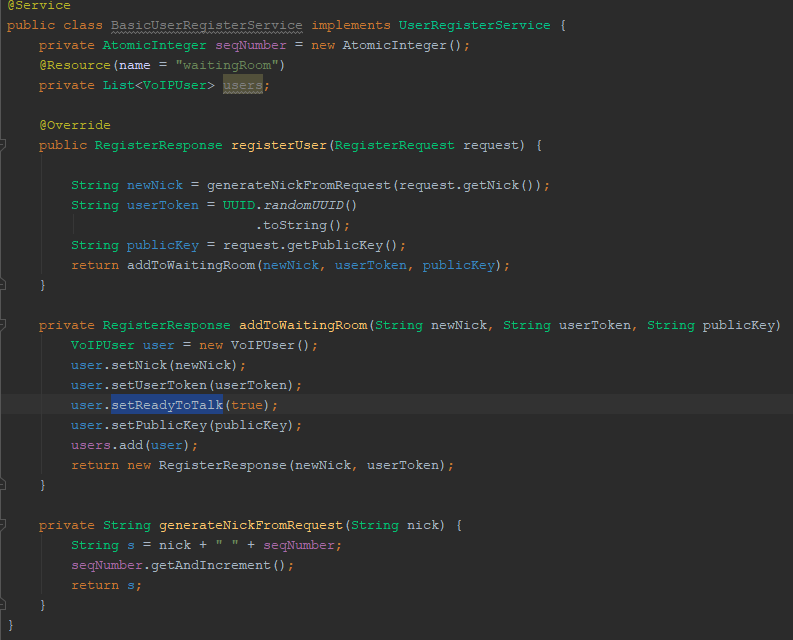
\includegraphics[width=\textwidth]{images/code1.png}
	\centering	
	\caption{\centering Kody serwisu zarządzającego użytkownikami i poczekalnią.}
\end{figure}

\subsection{ConnectionService}
\justy{Serwis odpowiedzialny za łączenie i rozłączanie użytkowników pośrednio wykorzystuje SessionService który zarządza dodatkowo sesjami użytkowników.}

\begin{figure}[H]
	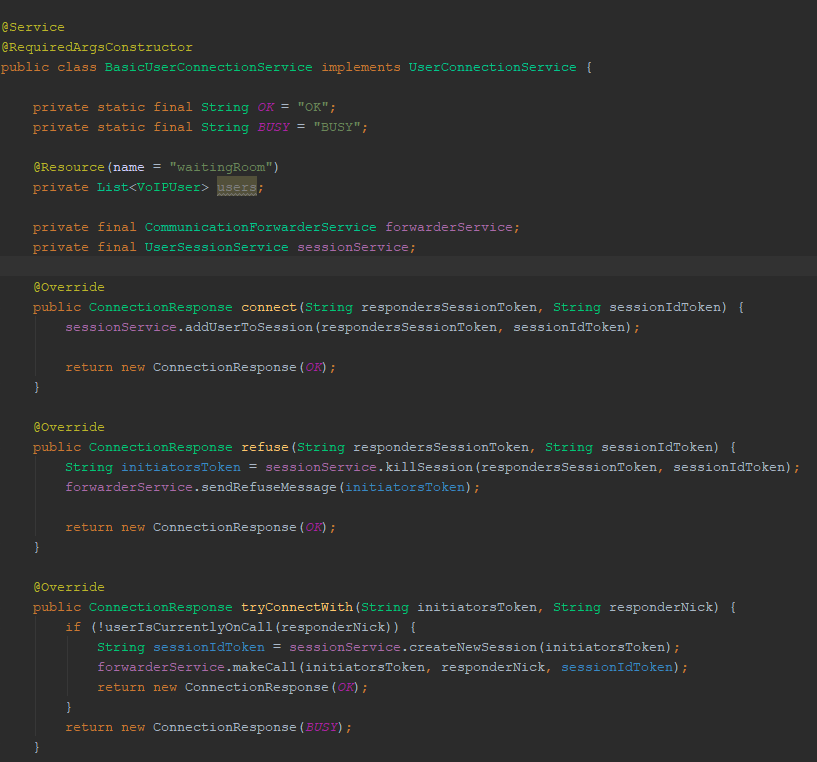
\includegraphics[width=\textwidth]{images/code2.png}
	\centering	
	\caption{\centering Klasa zarządzająca połączeniem użytkowników podczas próby rozmowy.}
\end{figure}